%!TEX root = ../thesis.tex
%*******************************************************************************
%****************************** Second Chapter *********************************
%*******************************************************************************

\chapter{Background}

% \ifpdf
    \graphicspath{{Chapter2/Figs/Raster/}{Chapter2/Figs/PDF/}{Chapter2/Figs/}}
% \else
%     \graphicspath{{Chapter2/Figs/Vector/}{Chapter2/Figs/}}
% \fi

\section{Properties of Blockchain Technologies}

The advent of cryptocurrencies made blockchains an overnight darling, set to make significant disruptions 
in several industries such as financial services, currency exchanges, supply chain management, retail 
advertising and identity management \citep{forbes2017industries}.

Impossible to collude: executed by transparent code, increase trust and enables reputation building for even new entrants to 
the education market
Protects learner: guaranteed records and rewards
% Scam? Reputation building? https://books.google.co.uk/books?id=jEsRVTbukyMC&lpg=PR5&ots=DKQbVRC8Yh&dq=high%20education%20assessment%20reputation&lr&pg=PA233#v=onepage&q=high%20education%20assessment%20reputation&f=false
Administration costs of higher education
Smart Contract: secure and cutting the middleman

Public v. Private 

Permissionless v. Permissioned

\citet{wust2017you} summarised  %https://eprint.iacr.org/2017/375.pdf


Characteristics of a blockchain ledger such as Hyperledger:
1. Shared Ledger: 
shared across education and government authorities
2. Smart Contract: 
Swan (2015, p.62) proposed that “rules embedded in learning smart contracts could automatically confirm the completion of learning modules 
through standardized online tests”.
3. Privacy: 
a. Appropriate Visibility
b. Transactions are secure, authenticated and verifiable
4. Consensus: All shared ledger parties agree to transactions

Openness and transparency of online courses and online assessments is encouraged: using an interpreted language, instead of a compiled 
one, to write the smart contract, so the actual code is visible on the blockchain and can be easily inspected
% Trust in Education Providers can be maintained the identity of any addition or modification to the record can be traced, records cannot 
be removed or altered
% Privacy of course participants is protected: events are publicly-accessible, but not publicly readable without a digital key
Resilient to loss of infrastructure: records are distributed over a network of participating computers

\section{Review of Relevant Education Research}

Identifying issues in traditional higher education today that a future system can better 
tackle is one of the objectives of this project. This informs the scope of the 
project and the design of the deliverables.

There is an abundant amount of pedagogy and learning method research, which focuses on the 
instruments and mode of delivery. These include methods such as "scaffolding", "constructivism", 
"problem-based learning", and "active learning" \citep{ali2005effective}. However, this 
research area is considered out of the scope of discussion for this project, which does not 
aim to provide new insight into ICT-enhanced pedagogies, nor will it be designed around any 
preferred pedagogies. This project is interested in representing components of e-learning, 
such as delivery, assessment, and record keeping in a more generic, general purposed manner.

\subsection{Assessments and Transparency}

Assessment is arguably the most important process in the business of education as it "drives what 
is learnt and taught" and "convert learning into credentials". \citep[p.160]{campbell2010digital}

\citet{brown1999assessment} summarised examples of popular sentiments learners held about both 
continuous assessments and traditional exams, such as:

\begin{enumerate}
    \item Assessment tasks do not increase students' want to learn, only their need to learn, promoting unhappiness;
    \item Invalid and unreliable marking due to speed or fatigue of assessors, plagiarism and unwanted collaborations, etc.;
    \item Sub-optimal levels of feedback after many types of assessments;
    \item Students feel forced into surface learning
    \citep[p.62-65]{brown1999assessment}
\end{enumerate}

The importance of assessments, coupled with popular unhappiness and mistrust amongst learners towards 
them, grows the tension between the teacher (or educational provider) and the learners.

\citet{suhre2013determinants} looked into motivation on study progress in a higher education setting by collecting data 
from 168 first-year university students for six months. The study found three main factors that motivates academic 
progress: intrinsic abilities, personal motivations such as a need to achieve or fear of failure, and transparency in 
exams and assessments.

Transparency here refers to both the clarity of assessment goals and the procedures for assessing these goals. 
It should be clear to learners what knowledge is required for a sufficient level of mastery. \citep{suhre2013determinants}
The difference this makes was significant:

\begin{itemize}
  \item Students' perceptions of degree programme organization and transparency of exams are also 
  significantly correlated with academic performance;
  \item Academic pressure is substantially influenced by the perceived transparency of assessments.
\end{itemize}

An improvement in the transparency of goals, procedures, knowledge required of assessments and an increase 
in feedback can directly tackle some of the negative sentiments listed above from \citet{brown1999assessment}, 
such as 1, 2 and 3.

\subsection{Personalisation in Education}

Cover personalisation broadly and in terms of curriculum (which modules to take, 
customised passing thresholds) which can be negotiated on the blockchain.
To be added if there is time for the project to cover this area.

\section{Literature Review in e-Learning}

E-learning has been growing as an industry and research area, and various standards have been devised. 
A review of these frameworks could provide valuable insights.

\subsection{e-Learning Systems}

\begin{figure}[!ht] 
    \centering    
    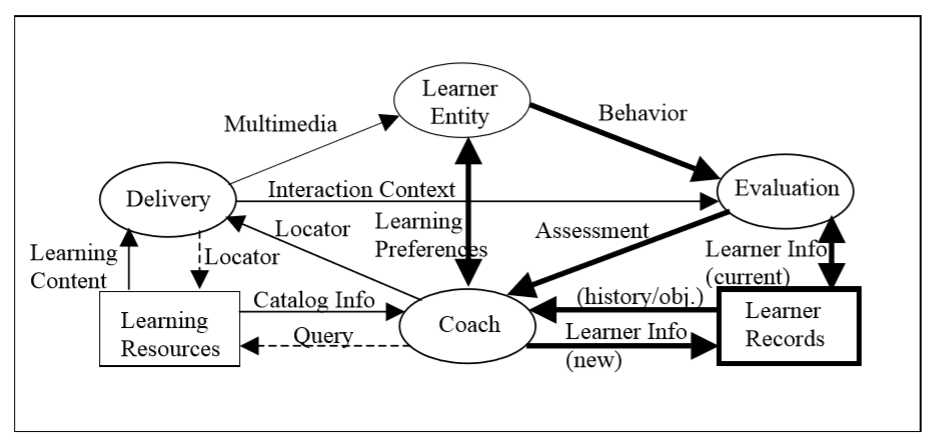
\includegraphics[width=1.0\textwidth]{LTSA}
    \caption[Learning Technology Systems Architecture]
        {Learning Technology Systems Architecture, IEEE P1484.1/D9 \citep{farance1999learning}}
    \label{fig:LTSA}
\end{figure}

IEEE P1484.1/D9: the Learning Technology Systems Architecture (LTSA) provides a valuable way of organising 
the scope and discussion in this project. It identified four main components: learner entity, coach, 
delivery and evaluation; and two main resources: learning resources and learner records (See figure \ref{fig:LTSA}).

Identifying the properties of a blockchain-based system that could improve these components is 
critical to this project. For example, the distributed, immutable storage of learner records could 
provide extra security.

\subsection{e-Learning Research Framework}

\citet{garrison2011learning} provided a framework for research and practice called the "Community 
of Inquiry (CoI)" framework, which included three main categories:

\begin{enumerate}
    \item Enhancing the social presence, such as collaborative learning
    \item Enhancing the cognitive presence, such as practical inquiry and critical thinking
    \item Enhancing the teaching presence, especially with asynchronous e-Learning (eg. pre-recorded lectures)
\end{enumerate}

A blockchain back-end could potentially provide experiential improvements in the above three categories as well. 
For example, smart contracts could enhance the social and teaching presence by facilitating teacher-learner, or 
learner-learner negotiations.

% \subsection{Self-Regulation and Motivation}

% There are several dimensions of self-regulation that will help a learner stay on an 
% e-Learning course or curriculum:

% \begin{table}[!ht] 
%     \caption{Self-Regulation and Motivation Strategies, adapted from \citep[p.189]{o2013web}}
%     \centering
%     \label{table:Self-regulation Dimensions}
%     \begin{tabular}{l c }
%         \toprule
%         Self-regulation Dimensions & Examples of Motivation Strategies \\ 
%         \midrule
%         Motives & Setting challenging but achievable goals \\ \hline
%         Methods of Learning & Summarisation, outline-formatted notes, \\
%         & interrogation and rehearsal, etc\\ \hline
%         Time Management & Prioritizing tasks, dealing with procrastination\\ \hline
%         Physical Environment & An environment conducive to learning\\ \hline
%         Social environment & Help seeking: knowing when help is needed,\\
%         & identifying sources of help, framing help request,\\
%         & evaluating help received\\ \hline
%         Performance & Observing and reflecting upon performance\\
%         & with short-term and long-term goals\\
%         \bottomrule
%     \end{tabular}
% \end{table}

% An e-learning programme should equip a learner with these self-regulation skills,
% and the e-learning system should provide tools that facilitate and enable the 
% motivation strategies.

\subsection{Security and Privacy}

The security of e-learning systems have also been a concern. For example, \citet{el2003privacy} noted that “while many 
advances have been made in the mechanics of providing online instruction, the needs for privacy and security have to-date 
been largely ignored. At best they have been accommodated in an ad-hoc, patchwork fashion.”

The consequences of cybersecurity breaches have also become more and more expensive. For example, when the General Data 
Protection Regulation (GDPR) comes into effect across Europe in May 2018, the maximum fine for poor practices and data 
breaches will be £17 million or 4\% of global turnover \citep{ico2017gdpr}.

The scale and severity of historic breaches of of internet services has been worrying. Most notably in the e-learning 
industry, the education platform Edmodo was hacked and 77M account details were lost and on sale on the dark 
web, endangering students, teachers and parents who are account holders \citep{opsecmonkey2017edmodo}.

The sizable threat and consequences makes a "security by design" and "privacy by design" approach for future e-Learning 
systems very important.
% The Information Commissioner's Office also encourages a "privacy by design approach" and 
% https://www.ipc.on.ca/resource/privacy-by-design/

\section{Existing Efforts in Blockchain for Education}

% chapter 1
% The potential of blockchain enabled systems in education has been noted by the community, with \citet[p.62]{swan2015blockchain} 
% proposing that “learning smart contracts could automatically confirm the completion of learning modules through standardized 
% online tests”. Appropriate configurations in permissions and visibility can also provide improved security and privacy to e-Learning.

\subsection{Blockcerts}

Blockcerts is an open standard for blockchain certificates led by MIT’s Media Lab. Education providers can use it to store 
the records of certifications they have awarded (See figure \ref{fig:blockcerts}). One bitcoin transaction is performed for 
every batch of certificates, with the certificates stored in the OP\_RETURN transaction field on the bitcoin blockchain. 
This is paid for by the certificate issuer. \citep{blockcerts2018}

\begin{figure}[!h] 
    \centering    
    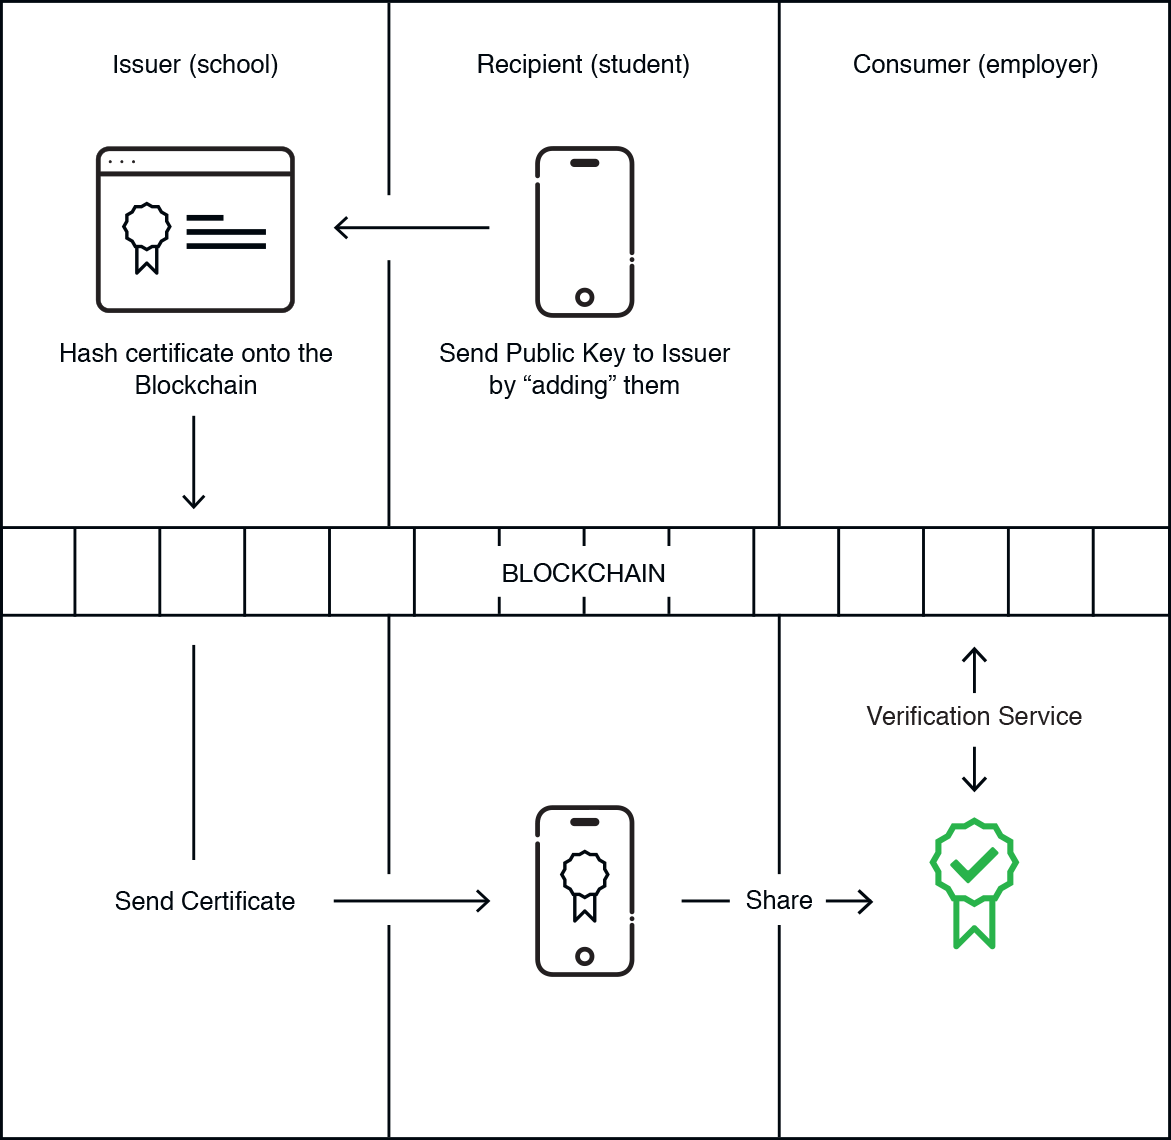
\includegraphics[width=0.7\textwidth]{blockcerts}
    \caption[How Blockcerts work]
        {How Blockcerts work \citep{blockcerts2018}}
    \label{fig:blockcerts}
\end{figure}

\subsection{Sony Global Education Blockchain}% https://blockchain.sonyged.com/

The Sony Global Education Blockchain is based on the Hyperledger project, an open source distributed ledger 
for businesses. It provides an application program interface (API) for developers at education institutes, 
allowing integration with third party applications. It aims to provide tamper-proof, secure storage of 
learning history data for institutions. \citep{sonyged2017}

\begin{figure}[!h] 
    \centering    
    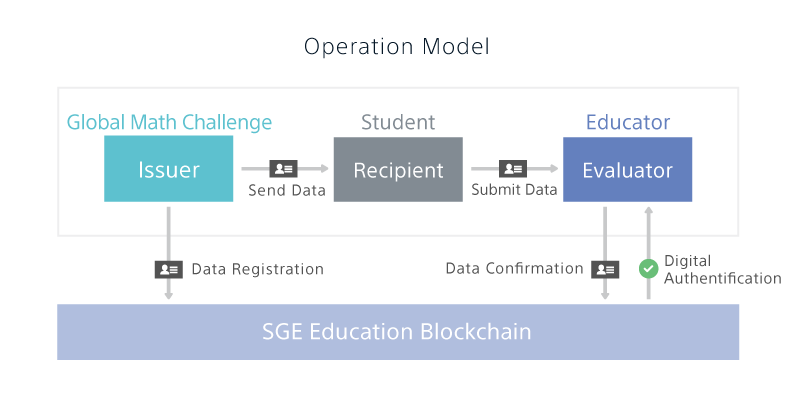
\includegraphics[width=0.7\textwidth]{sonyged}
    \caption[Sony Global Education Blockchain]
        {Operation Example of the Sony Global Education Blockchain \citep{sonyged2017}}
    \label{fig:sonyged}
\end{figure}

\subsection{OpenLearn Blockchain}% http://blockchain.open.ac.uk/

\begin{figure}[!h] 
    \centering    
    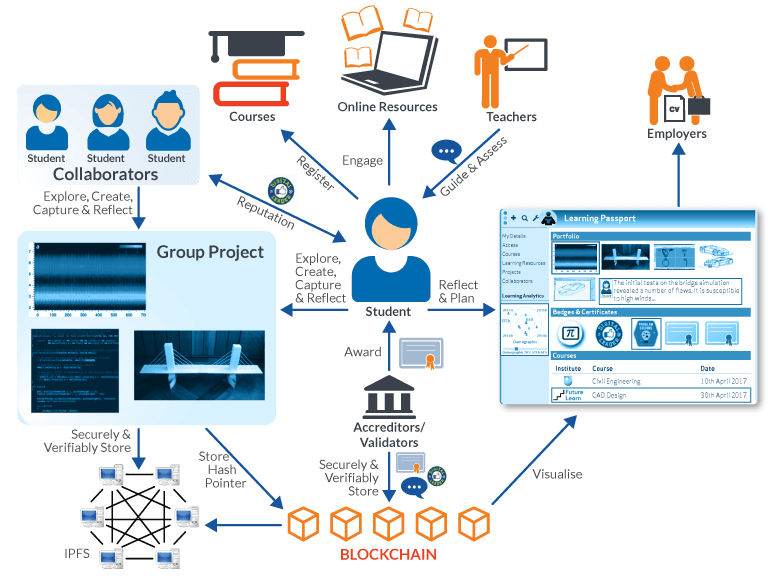
\includegraphics[width=0.95\textwidth]{openlearn}
    \caption[OpenLearn Blockchain scenario]
        {A typical education scenario with the OpenLearn Blockchain\citep{openlearn2018}}
    \label{fig:openlearn}
\end{figure}

The OpenLearn Blockchain project envisions the creation of blockchain based ePortfolios (See figure 
\ref{fig:openlearn}). They are currently demonstrating this with an experimental plugin for Moodle, 
a popular course management system, with which achievement badges can be stored on the Ethereum 
blockchain. This system currently allows students to register for courses and receive badges which 
can be viewed in a student Learning Passport. The transactions are peer-to-peer: in principle no 
host institution is required for the awarding of accreditation. \citep{sharples2016blockchain}

\subsection{Novelty of the proposed project}

\begin{figure}[!h] 
    \centering    
    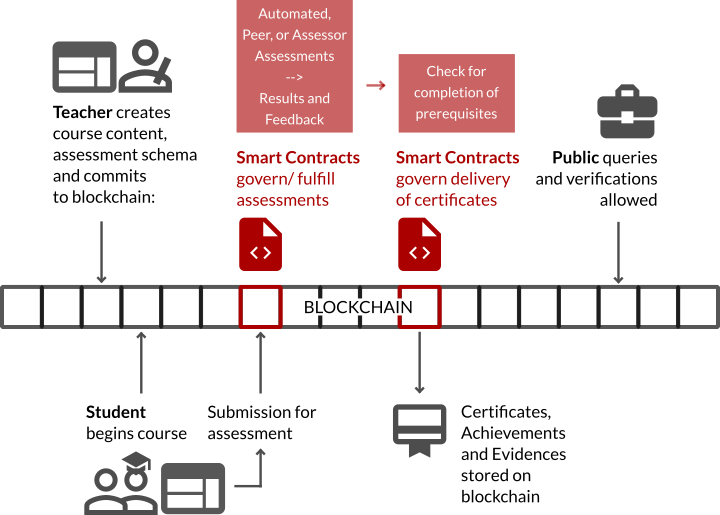
\includegraphics[width=0.95\textwidth]{moocon}
    \caption[How smart contracts automates assessments]
        {Original diagram providing a high level view of how the project proposes automating assessments 
        with smart contracts}
    \label{fig:moocon_assess}
\end{figure}

All of the above three notable efforts focus on identity management and record keeping for education. 
This project will aim to extend these efforts by proposing smart contracts that automate assessments 
(See figure \ref{fig:moocon_assess}) and deliver personalised curricula. 

The vision of this project will also be to create an e-Learning marketplace that teachers can use directly, 
instead of a blockchain network that education providers will have to consume through APIs. This makes for a 
lower cost of entrance in terms of technological know-how and investment.

\section{Overview of Blockchain Development Toolkits}

This project will involve the design of smart contracts for e-Learning transactions and building a demonstrator 
network and applications. A review of the popular blockchain implementations and development toolkits on the 
market is necessary. See table \ref{table:blockchainscomparison} for a overview and below for more commentary.

\begin{table}[!hb] 
    \caption{Comparison of key blockchain implementations, adapted from \citet{ibm2018hyperledger} and \citet{valenta2017comparison}}
    \centering
    \label{table:blockchainscomparison}
    \begin{tabular}{l c c c c}
        \toprule
        & Bitcoin & Ethereum & Hyperledger Fabric & R3 Corda\\ 
        \midrule
        Crypto- & bitcoin & ether, user-created & none, user-created & none \\ 
        currency & & cryptocurrencies & cryptocurrencies\\\hline
        Network & permissionless, & permissionless, & permissioned, & permissioned,\\ 
        & public & public or private & private & private\\\hline
        Transactions & anonymous & anonymous or & public or & \\ 
        & & private & confidential \\\hline
        Consensus & proof of work & proof of work & PBFT & PBFT\\ \hline
        Smart & none & yes (Solidity, & yes (chaincode) & yes (chaincode)\\ 
        Contracts & & Serpent, LLL) \\\hline
        Language & C++ & Golang, C++, & Golang, Java, & Kotlin, Java,\\
        & & Python & JavaScript & legal prose\\
        \bottomrule
    \end{tabular}
\end{table}

Bitcoin is included in the table only as a point of reference, building with the bitcoin 
blockchain is not considered for this project because of its lack of support for smart 
contracts (any kind of embedded logic or programmes).

\subsection*{Ethereum}

Ethereum is famous for its Turing-complete smart contracts capabilities

\subsection*{Hyperledger Fabric}

\subsection*{R3 Corda}

Built following use cases in the financial industry, 
% http://explore-ip.com/2017_Comparison-of-Ethereum-Hyperledger-Corda.pdf